\newcommand{\institut}{Institut f\"ur Energie und  Automatisiertungstechnik}
\newcommand{\fachgebiet}{Elektronische Mess- und Diagnosetechnik}
\newcommand{\veranstaltung}{Praktikum Messdatenverarbeitung}
\newcommand{\pdfautor}{\"Ozg\"u Dogan (326 048), Timo Lausen (325 411), Boris Henckell (325 779)}
\newcommand{\autor}{\"Ozg\"u Dogan (326 048)\\ Timo Lausen (325 411)\\ Boris Henckell (325 779)}
\newcommand{\pdftitle}{Praktikum Messdatenverarbeitung  Termin 5}
\newcommand{\prototitle}{Praktikum Messdatenverarbeitung \\ Termin 5}
\newcommand{\aufgabe}{}

\newcommand{\gruppe}{Gruppe: G1 Fr 08-10}
\newcommand{\betreuer}{Betreuer: J\"urgen Funk}

\input{../../packages/tu_header_8}
%\begin{document}

% \lstlistoflistings
\definecolor{darkgray}{rgb}{0.95,0.95,0.95}
\definecolor{darkolivegreen}{HTML}{01a801}
\definecolor{functionsBlue}{HTML}{32b9b9}
\definecolor{variableRed}{rgb}{1,0,0}
\definecolor{stringBrown}{HTML}{bc8e8e} % f geht nicht

\lstset{
        %\lstset{extendedchars=true} % Umlaute an der richtigen stelle und nicht am Anfang ausgeben
        %basicstyle=\footnotesize\ttfamily,
        basicstyle=\small,
        %
        inputencoding=utf8,
        %
        tabsize=4,
        showspaces=false,
        showtabs=false,
        showstringspaces=true, % no special string spaces
        %
        backgroundcolor=\color{darkgray}, % background
        stringstyle=\color{stringBrown}\fseries, % Strings
        keywordstyle=\color{functionsBlue}\bfseries, % keywords Blau
        identifierstyle=\color{variableRed}, % variablen
        commentstyle=\color{darkolivegreen}, %  comments
        %
        breaklines=true,
        %
        numbers=left,
        numberstyle=\tiny,
        stepnumber=1,
        numbersep=7pt,
        %
        frame=single,
        columns=flexible,
        %
        xleftmargin=-2cm,
        xrightmargin=-1.5cm,
        %
        language=Matlab
}


%---------------------------------------------------------------------
%---------------------------------------------------------------------
%---------------------------------------------------------------------


\section{Vorbereitungsaufgaben}
\begin{quote}
    
    \subsection{Vorbereitungsaufgaben zu Termin 5}
    \begin{quote}
    	
    	\subsubsection{FIR Filter entwerfen}
    	\begin{quote}
		    
			In der ersten Aufgabe sollte ein FIR-Filter entworfen werden, welches mit der MATLAB
			Funktion FIRFilterung realisiert wird. Hierbei handelt es sich um eine Funktion, die ein Eingangssignal mit Hilfe
			von Filterkoeffizienten filtert. Beides, das Eingangssignal sowie die Filterkoeffizienten werden der Funktion
			übergeben\vspace{1em}
			
			Die Funktion ist im Anhang dieses Protokolls angehängt.\vspace{1em}
			
			Um die funktionalität unserer Funktion zu überprüfen haben wir das Ergebnis unserer Funktion mit dem Ergebnis einer
			schon vorhandenen FIR-Filterfunktion verglichen.\\
			Dazu haben wir einen Deltaimpuls mit einer Reihe beliebig gewählter Filterkoeffizienten filtern lassen. Die entstandene Impulsantwort
			sieht folgendermaßen aus:
			
			\begin{figure}[H]
		            \centering
		                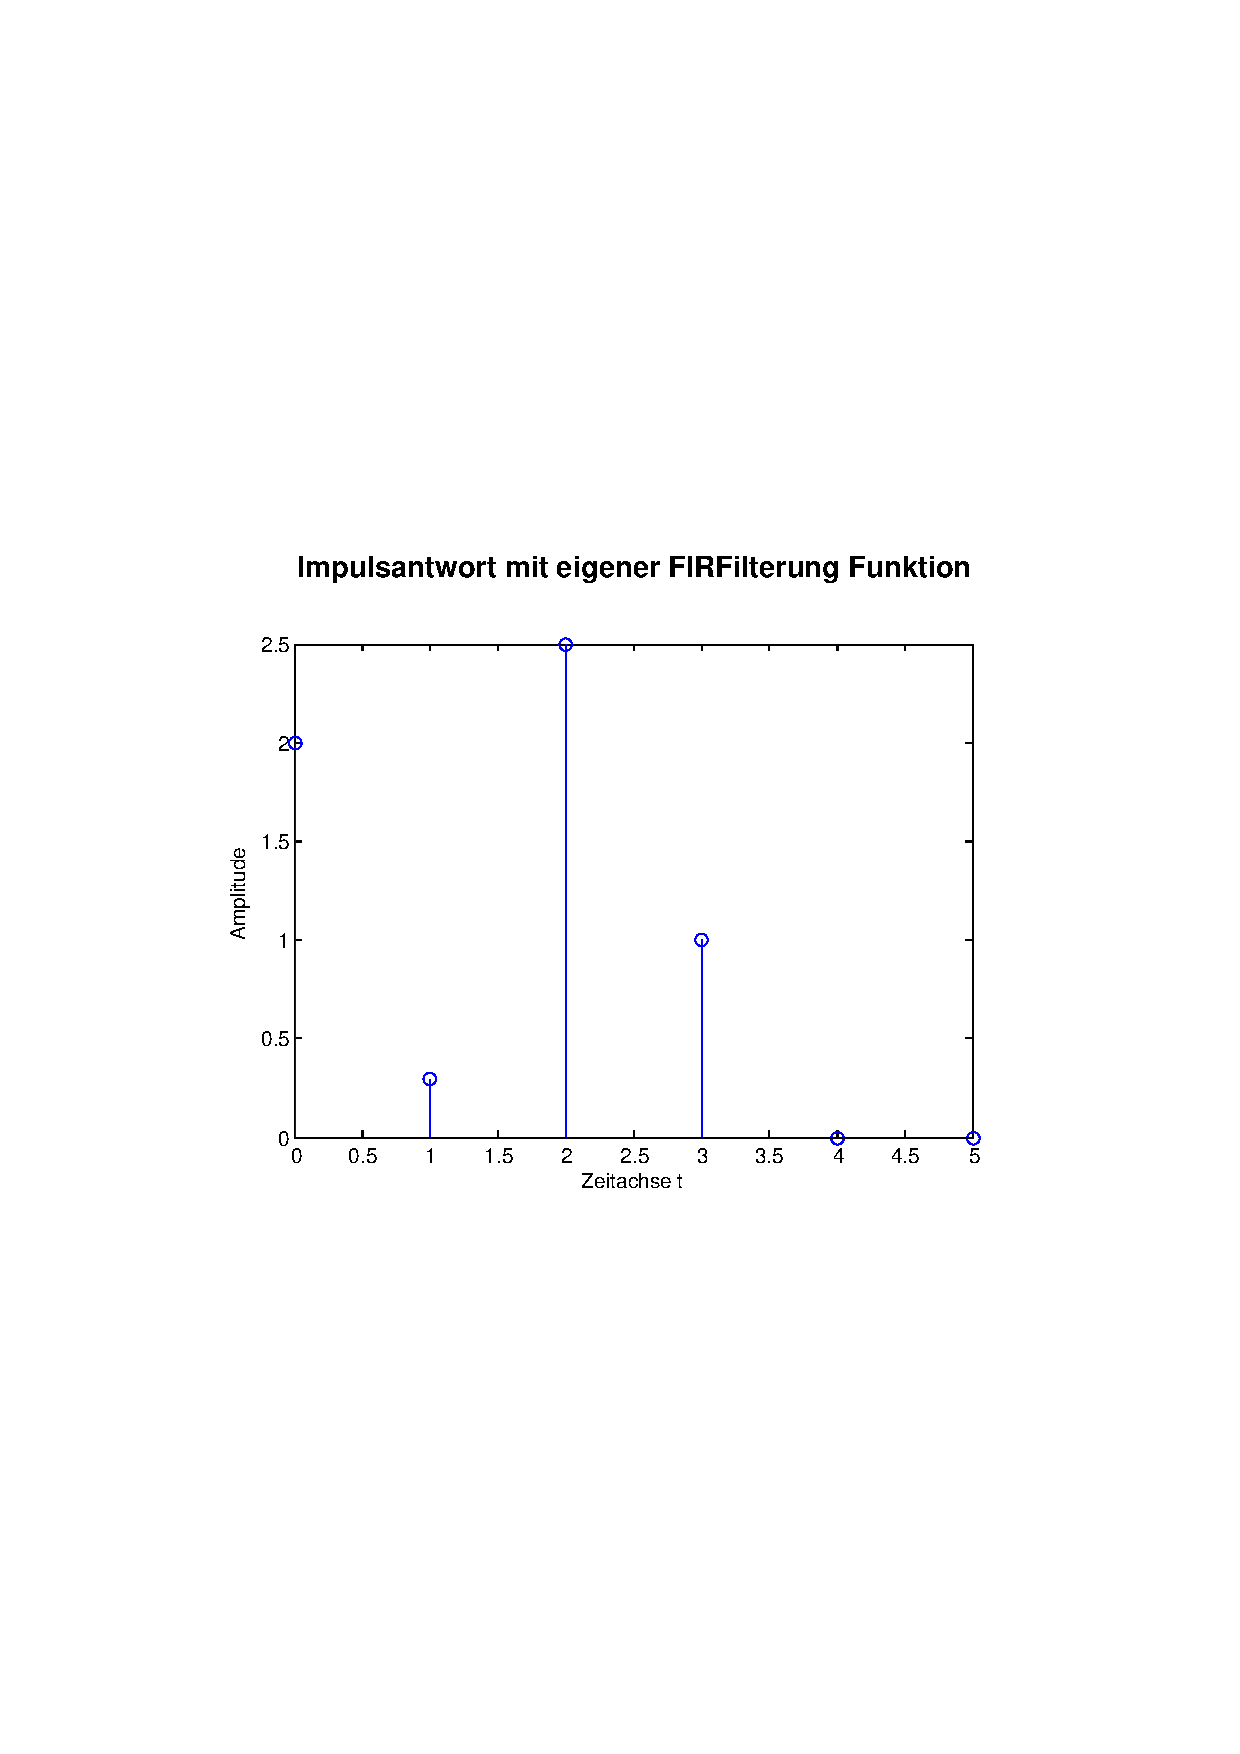
\includegraphics[scale=0.5, trim = 1cm 6cm 1.5cm 8cm,
		                clip]{./Bilder/Impulsantwort_aufgabe1}
		                    \caption{Impulsantwort mit belieben Filterkoeffizienten}
		                    \label{fig:./Bilder/Impulsantwort_aufgabe1}
		            \end{figure}
		            
			Übergeben wir deselben Deltaimpuls und dieselben Filterkoeffizienten der Matlab Funktion ``filter" erhalten wir diese
			Impulsantwort.
			
			\TODO{den nächsten satz nochmal besprechen und ggf einbauen} \\
			Hierbei ist zu beachten, d
			Das wichtige dabei ist es die Rückkopplungskoeffizienten der filter-Methode im ersten Eintrag zu $1$ und den
			Rest zu $0$ zu setzen, damit die Funktion des Filters weiter ohne Rückkopplung
			realisiert werden kann.\\
			
			\begin{figure}[H]
		            \centering
		                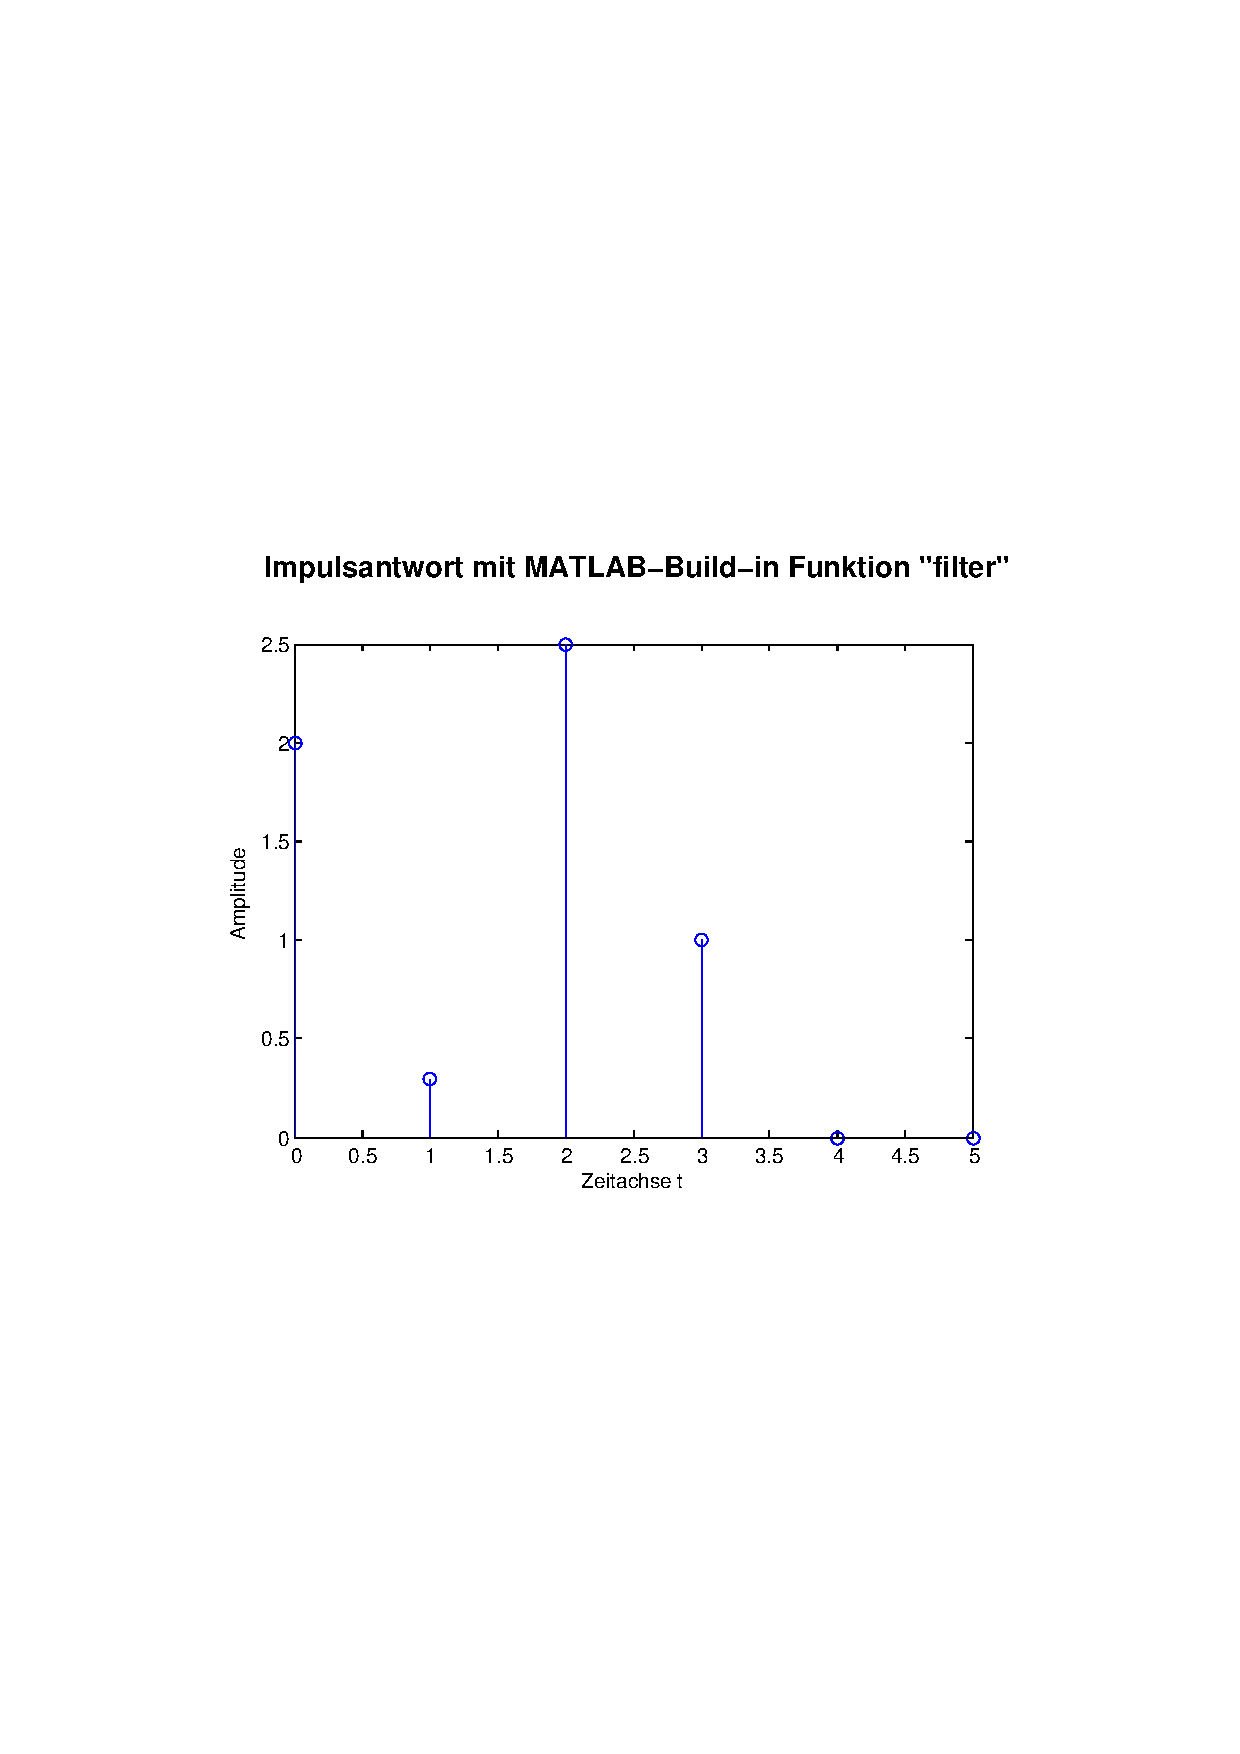
\includegraphics[scale=0.5, trim = 1cm 6cm 1.5cm 8cm,
		                clip]{./Bilder/Impulsantwort_aufgabe11}
		                    \caption{Impulsantwort mit anhand filter-Methode}
		                    \label{fig:./Bilder/Impulsantwort_aufgabe11}
		            \end{figure}
		       
		  \end{quote}   
		  
		  Es ist offensichtlich, dass die beiden Funktionen die selbe Impulsantwort besitzen. Daraus schließen wir, dass
		  unsere Funktion fehlerfrei funktioniert und wir sie im weiteren verlauf verwenden können.
		  
		  \subsubsection{FIR Filter nach der Fenstermethode entwerfen}
		  \begin{quote}
		            
		    In der nächsten Teil war die Aufgabe einen speziellen FIR-Filter zu Dimensionieren. Das sollten wir mit
		    Hilfe der Fenstermethode Schritt für Schritt eigenständig realisiert. Die Vorgabe war es,
		    ein Tiefpass zu bauen, welcher alle Frequenzanteile oberhalb von $1,5 kHz$
		    mit mindestens $60 dB$ dämpft und Frequenzanteile bis zu einer Grenzfrequenz
		    von $1 kHz$ mit maximal $3 dB$ dämpft. Die Abtastfrequenz des TP sollte
		    dabei $15 kHz$ betragen.\vspace{1em}
		     
		    Im ersten Schritt der Filterdimensionierung legen wir die Wunschfunktion $G_\omega (f)$ im Frequenzbereich fest,
		    die der Filter annehmen soll. In diesem Fall handelt es sich um einen Tiefpass.\\
		    Im zweiten Schritt transformieren wir diese Wunschfunktion in den Zeitbereich und erstellen damit die gewünschte
		    Impulsantwort. Über die Impulsantwort lassen sich später die Filterkoeffizenten ablesen.\\
            Da es sich bei unserer Wunschfunktion um einen Tiefpass handelt und dieser schon im Skript umtransformiert
            wurde nutzen wir diese gegebene Impulsfolge aus dem Skript.
		    
		    \begin{equation*}
            	\begin{split}
            		g_\omega(k) &= \int_{-f_g}^{f_g} G_\omega(f)e^{j2 \pi fkT} \mathrm df = \int_{-f_g}^{f_g} e^{j2\pi
            		f(kT-\tau)} \matrm df\\
            		g_\omega(k) &= \frac{sin(2\pi f_g (kT-\tau))}{\pi (kT-\tau)} \text{\ \ \ für \ } -\infty < k < \infty  
            	\end{split}
            \end{equation*}
		     
		    Da es sich hierbei jedoch um eine Unendliche Reihe handelt und die Impulsantwort des FIR-Filters endlich sein muss
		    legen wir im dritten Schritt noch ein Fenster über diese Reihe. In die Funktion Implementiert haben wir dazu ein
		    Hanningfenster, ein Blackmanfenster, ein Hammingfenster und ein Rechteckfenster.\\
		    
		    Diese Schritt haben wir in den Funktionen ``getFIRTiefpass'' und ``Testfunktion'' realisiert, die im Anhang zu
		    sehen ist.
		    
		    In der Funktion ``Testfunktion'' haben wir nun die gewünschte Grenzfrequenz und die Filterordnung vorgegeben, uns
		    die passenden Filterkoeffizienten sowie die Impulsantwort dieses Filters mit Hilfe der Funktion
		    ``FIRFilterung'' ausgeben lassen. Anschließend haben wir den Amplituden und Phasengang geplottet und
		    kontrolliert, ob das Filter mit der angegebenen Ordnung und Fensterung die Vorgaben erfüllt. Falls nicht haben wir
		    so lange die Filterordnung oder die Fensterung verändert, bis die Vorgaben erfüllt waren.\\
		    Am Ende haben wir eine Filterordnung von $85$ bei einem Hanningfenster. Der dazugehörige Frequenzgang sieht
		    folgendermaßen aus:
		    
		    \begin{figure}[H]
            \centering
                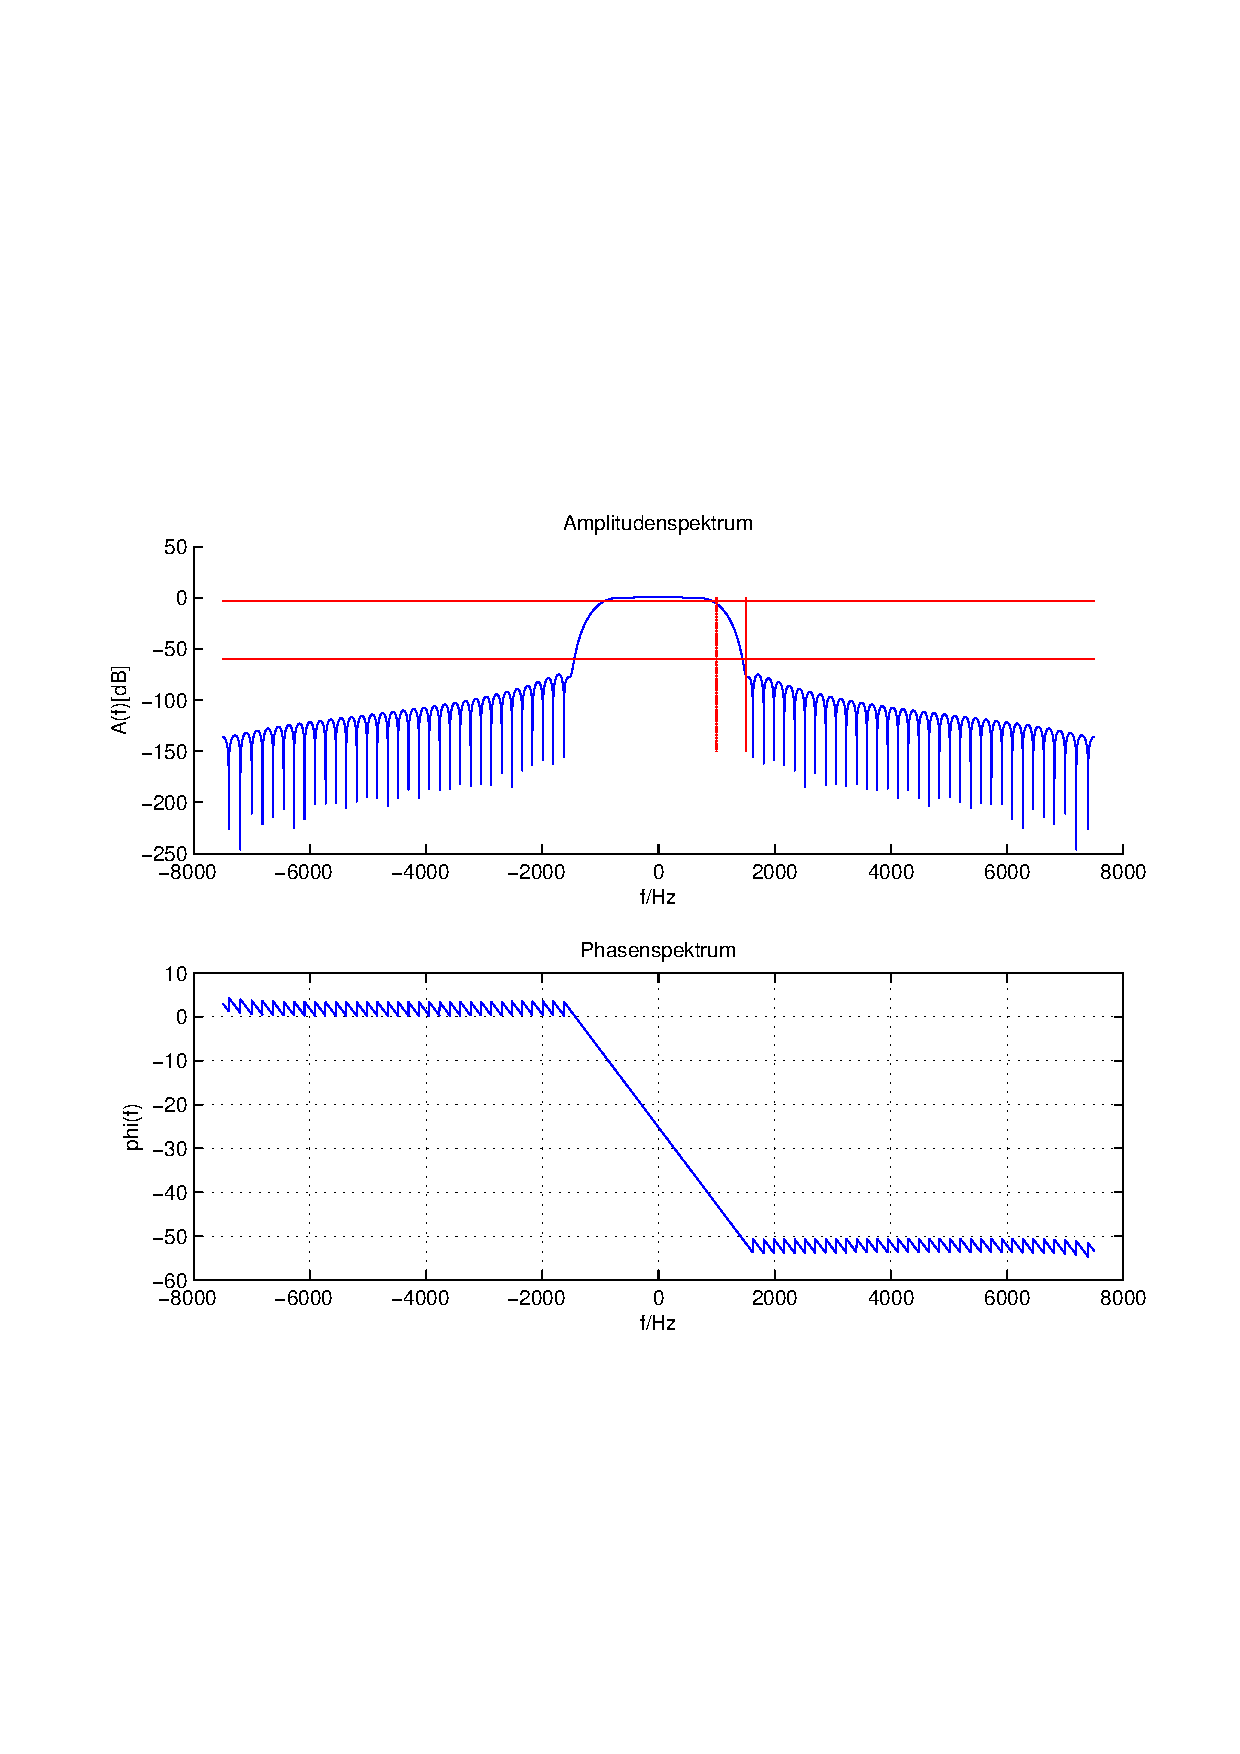
\includegraphics[scale=0.7, trim = 1cm 6cm 1cm 8cm, clip]{./Bilder/Amplitudengang_FIRFilter}
                    \caption{Amplitudengang FIR-Filter}
            \end{figure}
    
		    
		            
		            
		  \end{quote}          
		            
		  \subsubsection{Nachabtastung}
		  \begin{quote}
		            
		    Nun wurde eine Funktion entworfen, mit der sowohl die digitale Filterung als
		    auch das Nachabtasten des Signals realisiert wird. Dabei wird nur jeder
		    fr-ter Wert weiterhin übernommen.  
		 
		  \end{quote}
		  
		  \subsubsection{Verzicht auf analoges Anti-Aliasing-Filter?}
		  \begin{quote}
		  
		  Zuletzt sollte eine Antwort auf die Frage gegeben werden, ob durch den
		  Einsatz eines digitalen Filters ganz auf die Verwendung eines analogen
		  Anti-Aliasing Filters verzichtet werden kann. Die Antwort lautet nein. Durch
		  korrekte Anpassung des digitalen Filters mit ausreichend hoher Ordnung kann zwar 
		  Aliasing beim digitalen Filtern vermieden werden, doch braucht man bei der
		  Digitalisierung des Signals vor der Filterung einen Schutz vor Aliasing,
		  welcher nur durch ein analoges Anti-Aliasing Filter möglich ist.
		  
		  \end{quote}
	
	\end{quote}%Ende Vorbereitungsaufgaben Termin 5
	
	
    \subsection{Vorbereitungsaufgaben zu Termin 6}
    \begin{quote}
    	
    	Nachdem wir uns mit dem vorgegebenen Tutorial über Fix-Point Arithmetic in
    	C beschäftigt hatten, sollten folgende Aufgaben zur Vorbereitung des 6.
    	Termins angefertigt werden.
    	
    	\subsubsection{Beschreibung der Funktion filterFIR}
    	\begin{quote}
    	Zuerst wurde die vorgegebene Funktion filterFIR in ihrer Funkionsweise
    	erklärt:\\ 
    	Die Funktion filterFIR filtert ein gemessenes Signal. Bei Aufruf
    	wird der n-te Eintrag des gefilterten Signals ausgegeben und der Index incrementiert.\\
    	Die Filterfunktion ist mit einer for-Schleife realisiert. Folgende Schritte werden innerhalb eines Durchlaufs
    	durchgeführt.\\
    	Zu Beginn wird der n-te Messwert aus dem Buffer geholt. Dieser ursprüngliche Messwert hat 10 Bit und keine
    	Nachkommastellen. Um 6 weitere Nachkommastellen zu erhalten wird dieser um 6 Stellen nach links geshiftet. Im
        nächsten Schritt wird der Wert mit dem entsprechenden Filterkoeffizenten multilpliziert. Alle Filterkoeffizenten
        sind 16 Bit groß und haben 15 Nachkommastellen. Bei der Multiplikation
        von zwei 16 Bit Zahlen ergibt sich eine 32 Bit Zahl. Das Ergebniss
        besitzt nach der Multiplikation 21 Nachkommastellen. Für die weitere Rechnung werden die letzten 16 Nachkommastellen vernachlässigt. 
        Die Ergebnisse aller Multiplikationen werden zum Endergebniss
        aufaddiert. Daraus resultiert das gefilterte Signals an der Stelle n.\\
        Nach Vollendung wird der n-te Messwert aus dem Speicher gelöscht.
        Dadurch wird beim nächsten Aufruf der n+1 -te Messwert gefiltert.\\
        Abschließend werden die noch verbleibenden 5 Nachkommastellen abgeschnitten und das gerundete Ergebniss
        zurückgegeben.
        
		\end{quote}
		
		\subsubsection{Umwandelung der Filterkoeffizienten in das (0,15) Format}
		\begin{quote}
		
		Die im vergangenem Praktikum eingestezten Filterkoeffizienten sollten nun in
		das Q($0,15$) umgewandelt werden. 
		\TODO{wie genau haben wir das gemacht?}
		Anschließend verwendeten wir die Funktion exportCoeff() aus der Code-Vorgabe,
		um die umgewandelten Koeffizienten in eine C-Header Datei filter\_coeff.h zu
		exportieren. Danach wurde mit dieser Datei die gleichnamige Datei aus dem
		AVRStudio-Projekt ersetzt und die von uns gewählte Ordnungszahl im Header
		filter.h in die Konstante FILTER\_ORD eingesetzt. 
		
		\end{quote}
		
		\subsubsection{Methode filterFIRDecim implementieren}
		\begin{quote}
		
		Zuletzt sollte in der Datei filter.c die Methode filterFIRDecim implementiert
		werden. Diese Methode dient, wie die MATLAB Funktion aus dem 5. Termin zur
		digitalen Filterung und einer folgenden Abtastung. Die Abtastfrequenz sollte
		ein fünftel der ursprünglichen Abtastfrequenz betragen. Das Ergebnis dieser
		Aufgabe ist in den Codes zu sehen.
		
		\end{quote}
	
	\end{quote}%Ende Vorbereitungsaufgaben zu Termin 6	
\end{quote}%Ende Vorbereitungsaufgaben

\section{Durchführungen}
\begin{quote}
		
		\subsection{Durchführung zu Termin 5}
		\begin{quote}
			
			Im praktischen Teil des 5. Labortermins, sollte untersucht werden, wie die
			Abtastrate eines Signals durch Nachabtastung (Dezimation) verringert werden
			konnte.
			
			\subsubsection{Aufnahme eines Rechtecksignals}
			\begin{quote}
			
			Zuerst sollte ein Rechtecksignal aufgenommen werde, welche eine Frequenz von
			$110 Hz$ besaß. Die Abtastrate betrug $15 kHz$ und es wurde ein analoges
			Anti-Aliasing Filter verwendet. Danach wurde das Amplitudenspektrum des
			Signals bestimmt und bis zu einer Frequenz von $1 kHz$ geplottet. 
			
			\end{quote}%Ende Aufnahme eines Rechtecksignals
			
			\subsubsection{Dezimation des Rechtecksignals}
			\begin{quote}
			
			Nun wurde eine Dezimation durchgeführt, in dem das Signal mittels eines MATLAB
			Skriptes nochmal mit einer Frequenz von $3 kHz$ abgetastet wurde. Somit
			erhielten wir jeden fünften Wert aus dem aufgenommenen Signal und konnten
			die die restlichen Werte verwerfen, wodurch die Datenmenge deutlich
			verkleinert wurde. Nach der Abtastung wurde erneut das Amplitudenspektrum
			ermittelt, bis $1 kHz$ dargestellt und mit dem Amplitudenspektrum aus der
			vorherigen Aufgabe verglichen.
			
			\end{quote}%Ende Dezimation des Rechtecksignals
			
			\subsubsection{digitale Filterung des Rechtecksignals}
			\begin{quote}
			
			Als nächstes wurde das Rechtecksignal mit dem in der Vorbereitungsaufgabe
			entworfenem digitalen Filter (zunächst ohne Dezimation) gefiltert und manuell
			mit der Abtastrate von $3 kHz$ dezimiert. Danach wurde wieder das
			Amplitudenspektrum bis $1 kHZ$ gebildet und mit den Ergebnissen aus den
			vorherigen Aufgaben verglichen.
			
			\end{quote}%Ende digitale Filterung des Rechtecksignals
			
			\subsubsection{Testen der Funktion DecimFilt}
			\begin{quote}
			
			Zuletzt haben wir die ebenfalls in der Vorbereitungsaufgabe entworfene
			Funktion DecimFilt auf das aufgenommene Rechtecksignal angewendet, wodurch das
			Signal automatisch erst gefiltert und dann mit der Abtastrate von $3 kHz$
			dezimiert wurde. Wieder wurde das erzielte Amplitudenspektrum mit den anderen
			Amplitudenspektren verglichen.
			
			\end{quote}%Ende von Testen der Funktion DecimFilt

		\end{quote}%Ende der Durchführung von Termin 5
		
		\subsection{Durchführung zu Termin 6}
		\begin{quote}
		
			\subsubsection{Aufnahme des Amplitudenfrequenzgangs}
			\begin{quote}
			
			Zunächst sollte im Praktikum der Amplitudenfrequenzgang des im
			Microcontroller implementierten FIR-Filters im Bereich von $0$ bis $15 kHz$
			aufgenommen werden. Dies verwirlichten wir, indem wir von $0 kHz$ angefangen
			den Effektivwert des gefilterten Signals aufzeichneten , um ihn dann im Bezug
			zur Frequenz zu plotten.
			\TODO{welches Eingangssignal wurde nochmal gefiltert? sinus?}
			Dieser aufgenommene Frequenzgang wurde mit dem in MATLAB berechneten
			Frequenzgang verglichen. 
			
			\end{quote}
			
			\subsubsection{Aufnahme eines Rechtecksignals mit zwei Abtastfrequenzen}
			\begin{quote}
			
			Nun wurde ein Rechtecksignal mit einer Frequenz von $110 Hz$ aufgenomemn.
			Dieses Signal wurde beim ersten Mal mit $3 kHz$ und beim zweiten Mal mit $15
			kHz$ abgetastet. Als analoges Anti-Aliasing Filter nutzen wir die blaue
			Wandler-Box, auf eine digtale Filterung sollte verzichtet werden.  
			
			\end{quote}			
			
			\subsubsection{digitale Filterung und Dezimation des Rechtecksignals}
			\begin{quote}
			
			Das gleiche, mit $15 kHz$ abgetastete Rechtecksignal sollte als nächstes
			zusätzlich digital gefiltert und mit $3 kHz$ dezimiert werden. Um die
			Nachabtastung realisieren zu können, mussten wir bei dem Aufruf der Funktion
			ucAnalogRead, welchen wir aus den Vorgaben entnommen haben, den Parameter für
			die Dezimierung auf 'ON' setzen. Außerdem war zu beachten, dass die Parameter
			SampleRate und NumSamples sich auf die Nachabtastung bezogen und
			dementsprechend angepasst werden mussten. 
			
			\end{quote}
			
			\subsubsection{Vergleich des Rechtecksignals mit und ohne digitale Filterung
			und Nachabtastung} 
			\begin{quote}
			
			In dieser Aufgabe sollten die aufgenommenen Rechtecksignal ohne und mit der
			digitalen Filterung und Nachabtastung im Zeit- und Frequenzbereich
			miteinander verglichen werden. Um Unterschiede besser wahrnehmen zu können,
			stellten wir beide Ergebnisse bis zu einer Frequenz von $1 kHz$ dar. Die
			Plots, sowie die sichtbaren Unterschiede sind in der Auswertung zu sehen. 
			
			\end{quote}
			
			\subsubsection{Zusatzaufgabe}
			\begin{quote}
			
			In der Zusatzaufgabe soll die Zeit gemessen werden, die filterFIRDecim() für einen Durchlauf
            benötigt. In einem Durchlauf wird eine stelle des messsignals gefiltert und gespeichert. Die vier
            nachfolgenden Messwerte werden gelöscht.
			
			Zuerst muss die Funktion filterFIRDecim() modifiziert werden. Vor Beginn des eigendlichen
            Durchlaufs wird der Port-Pin PC2 auf high gesetzt. Anschließend wird die Funktion normal
            ausgeführt. Vor Beendigung wird der Pin PC2 wieder auf low gesetzt. Also ist wird für die
            Dauer eines Durchlaufs ein High-Impuls generiert. Dieser kann mit dem Oszilloskop gemessen
            werden.\\
            
            \begin{figure}[H]
            \centering
                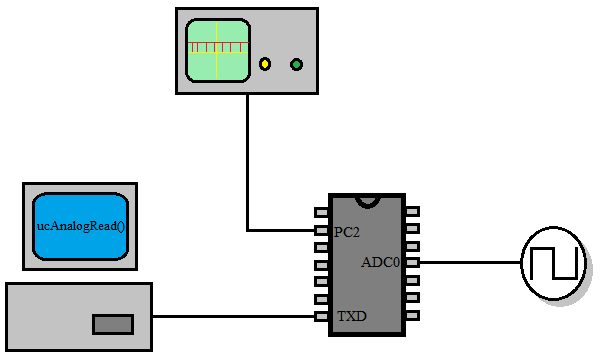
\includegraphics[scale=0.7, trim = 0cm 0cm 0cm 0cm, clip]{./Bilder/Zusatz.png}
                    \caption{Messung der Dauer von filterFIRDecim()}
            \end{figure}
        
            Der Funktionsgenerator wird an den Sensorknoten angeschlossen. Das Oszilloskop wird an den  
            Pin PC2 angeschlossen, um die Impulse messen zu können.
        			
			\end{quote}
			
			\end{quote}%Ende der Durchführungen von Termin 6
		
\end{quote}%Ende Durchführungen


%--------------------------------------------------------------------
%--------------------------------------------------------------------
\section{Auswertung}
\begin{quote}
	\subsection{Auswertung Termin 5}
    \begin{quote}
        \subsubsection{Auswirkung von Dezimation}
		\begin{quote}
			Es wird ein $110Hz$ Rechteck aufgenommen. Die Abtastrate beträgt $15kHz$. um Allaising zu
            vermeiden, wurde ein Antiallaisingfilter ("die blaue Box") verwendet. Anschließend wird das
            Amplitudenspektrum bestimmt und geplottet.\\
        
            \begin{figure}[H]
            \centering
                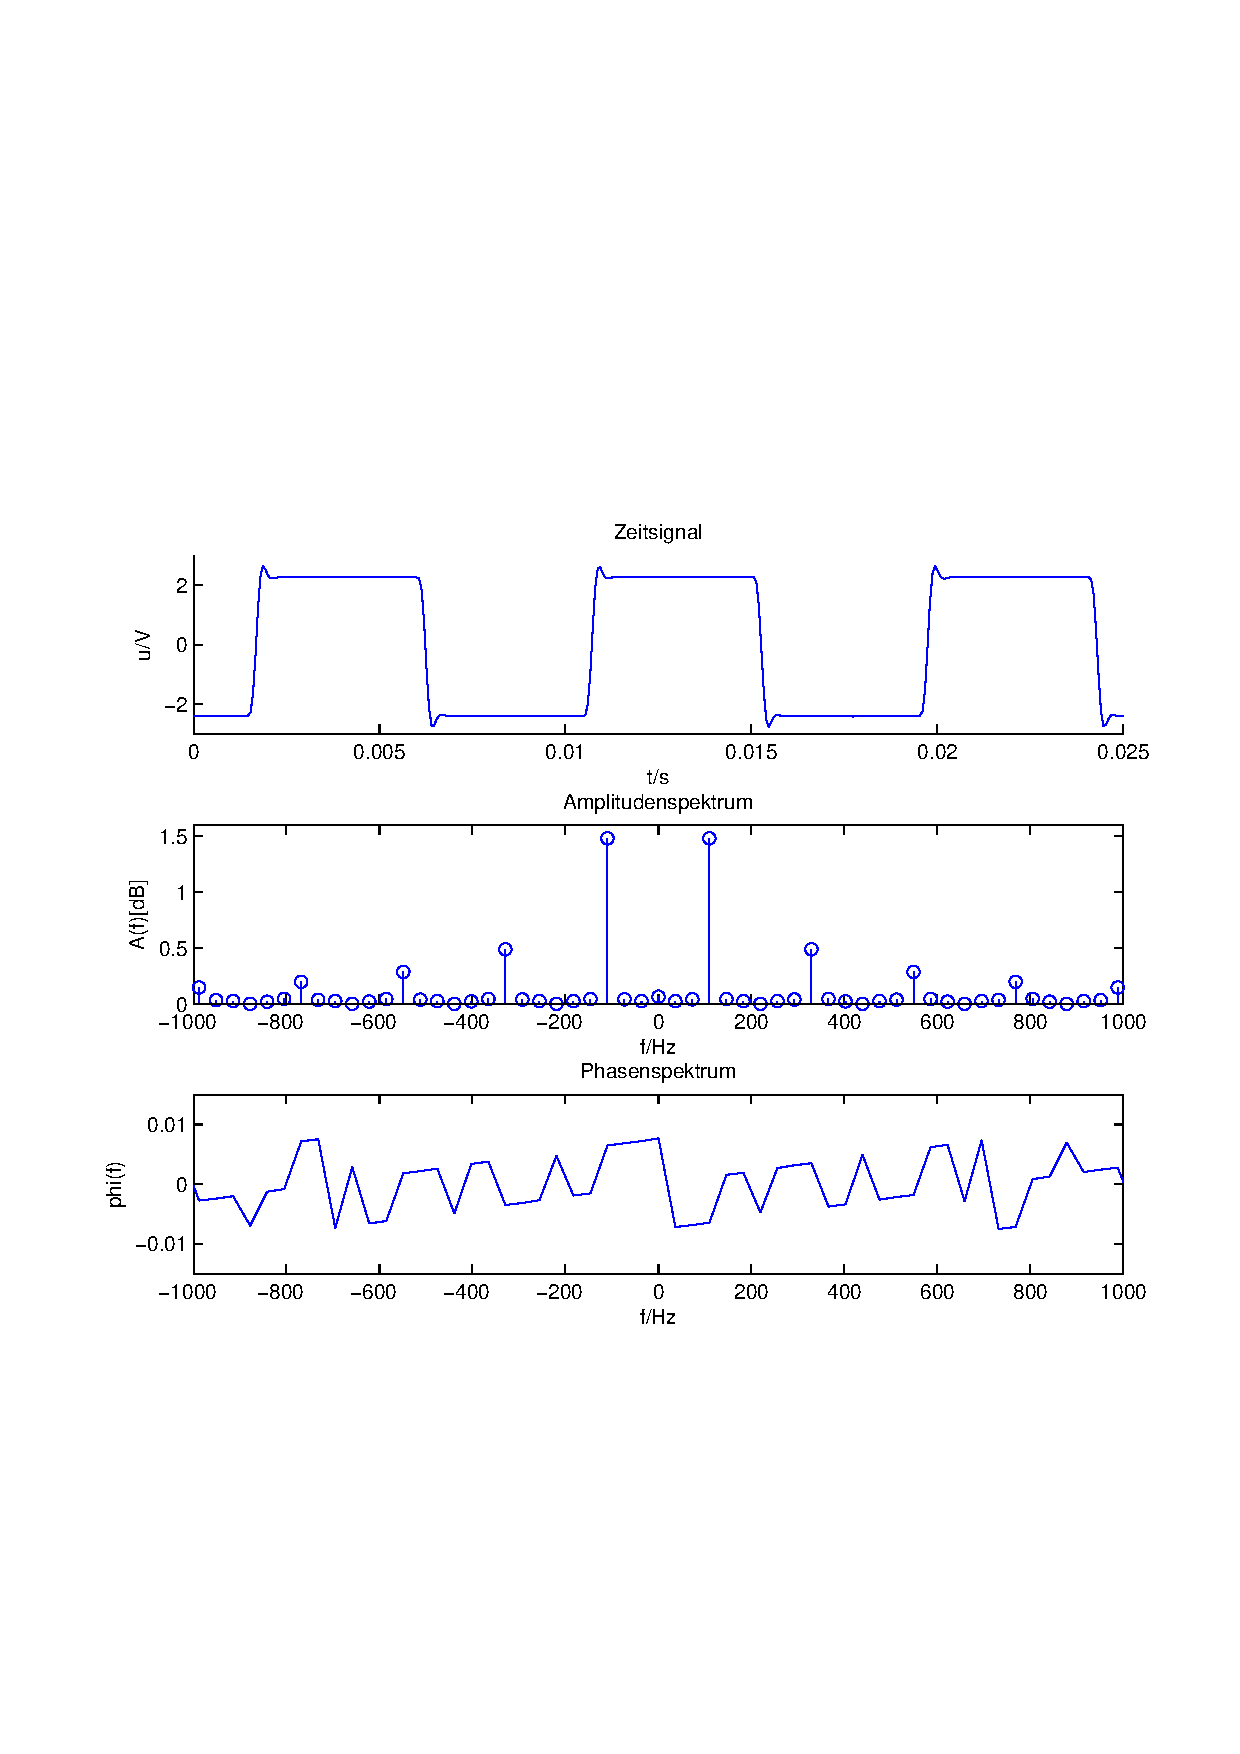
\includegraphics[scale=0.7, trim = 1.5cm 6.5cm 1cm 7.5cm,
                clip]{./Bilder/rechteck_100Hz_15kHz_frequenzbegrenzung.pdf}
                   \caption{aufgenommener Rechteck und sein Spektrum, auf 1kHz begrenzt}
            \end{figure}
    
        
            Das Spektrum sieht wie erwartet aus. Die Spektrallinien sind klar zu
            erkennen. Die kleineren Amplituden um die Spektrallinien herum sind minimale Oberwellen, da perfekte Rechtecke mit der
            Messkette nicht erfasst werden können. Dennoch ist das Messsignal sehr gut angenähert.\\
            Nun wird eine Nachabtastung (Dezimation) durchgeführt. Die Nachabtastung erfolgt mit $3kHz$. Dies
            läuft effektiv darauf hinaus das ein Messwert gespeichert und die folgenden vier gelöscht werden.
            Nach der Nachabtastung ist also nurnoch ein fünftel der Messwerte vorhanden.\\
            Auch das nachabgetastete Spektrum wird geplottet.
            
            \begin{figure}[H]
            \centering
                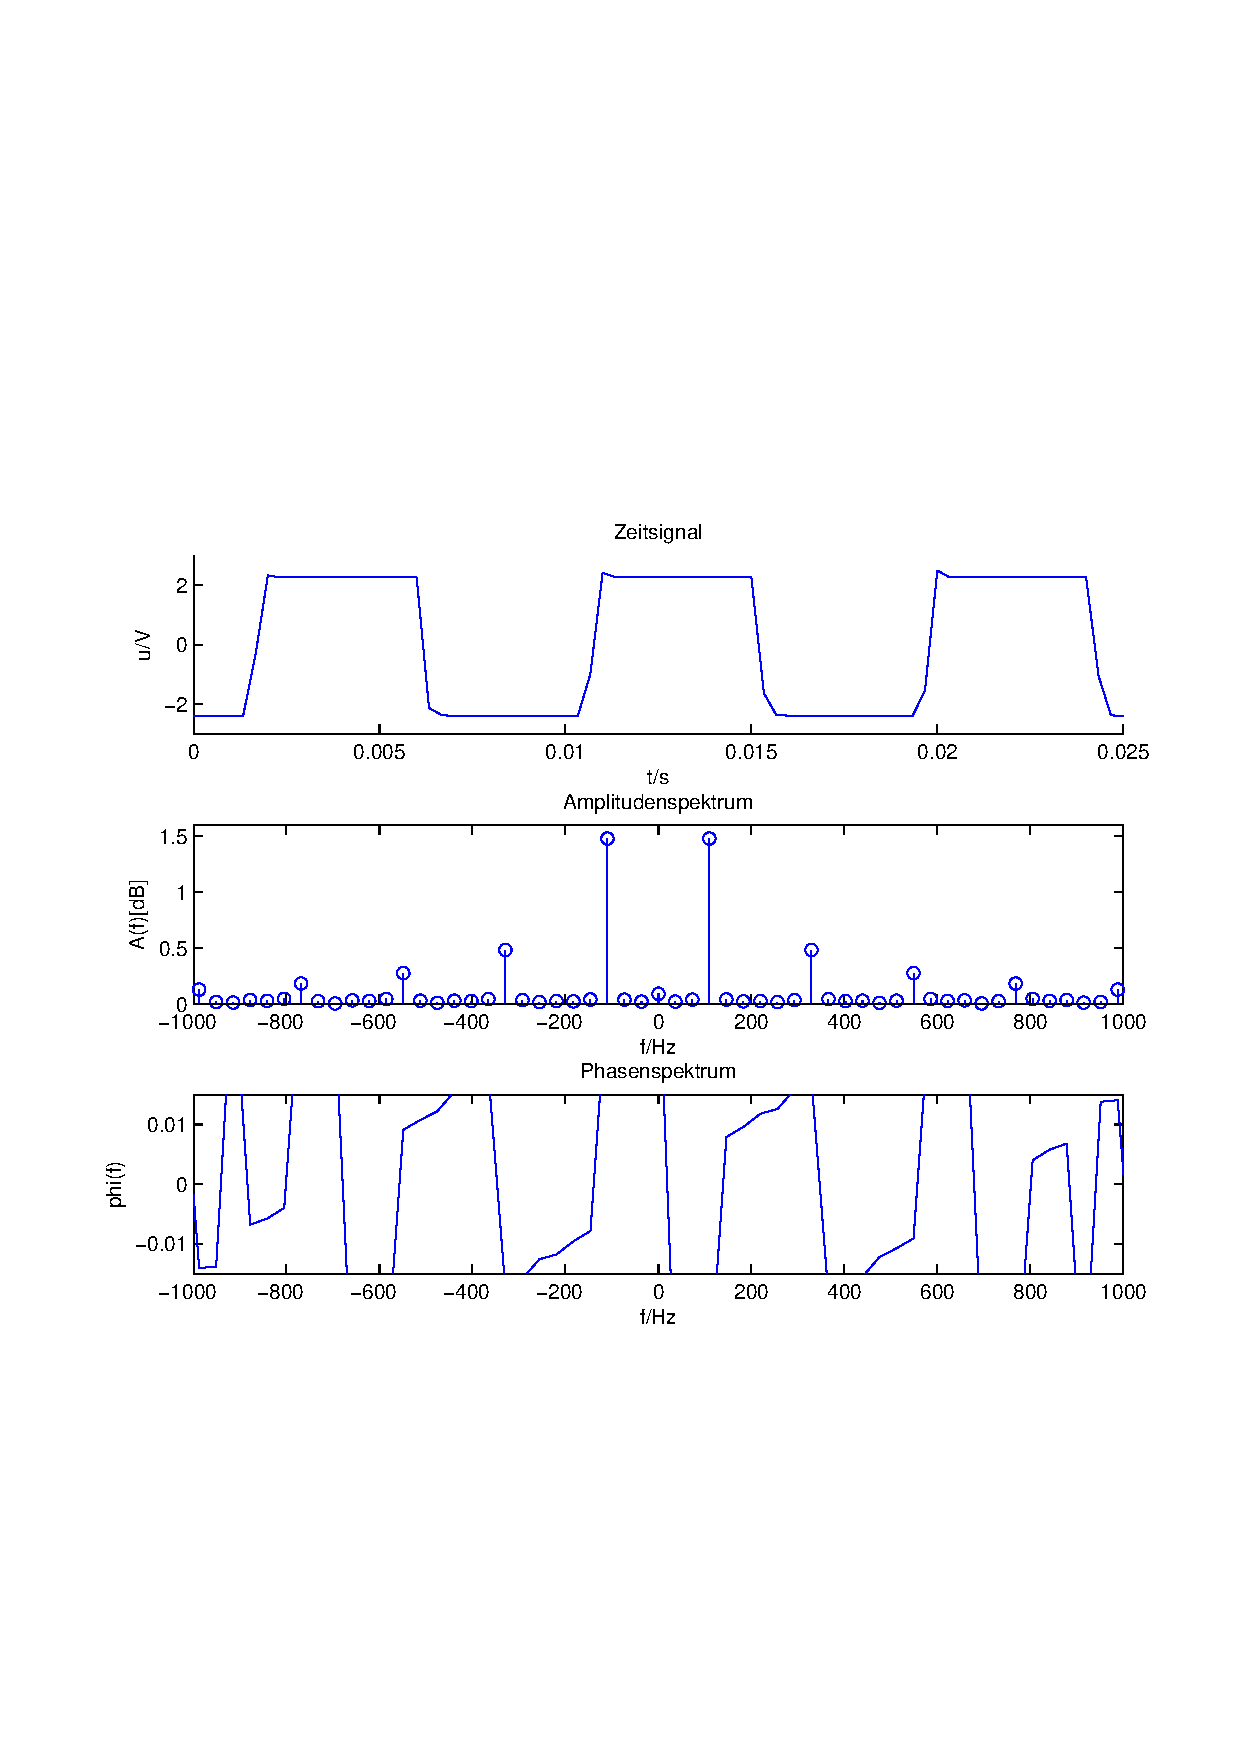
\includegraphics[scale=0.7, trim = 1.5cm 6.5cm 1cm 7.5cm,
                clip]{./Bilder/rechteck_100Hz_15kHz_3kHz_nachabgetastet_frequenzbegrenzung.pdf}
                    \caption{aufgenommener Rechteck nach der Nachabtastung}
            \end{figure}
  
            Bei einer diskreten Fourirtransformation erhält man für das Frequenzspektrum genau so viele
            Stützstellen, wie das Signal Abtastpunkte hat. Daher muss das nachabgetastete Signal nur ein    
            Fünftel der Spektrallinien haben.\\
            Auf dem Plot scheint es so, das sich die Anzahl der Spektrallinien nicht geändert hat. Die Änderung 
            wird aber klar, wenn man beide Spektren mit unbegrenzter Frequenzachse plottet.
            
            \begin{figure}[H]
            \centering
                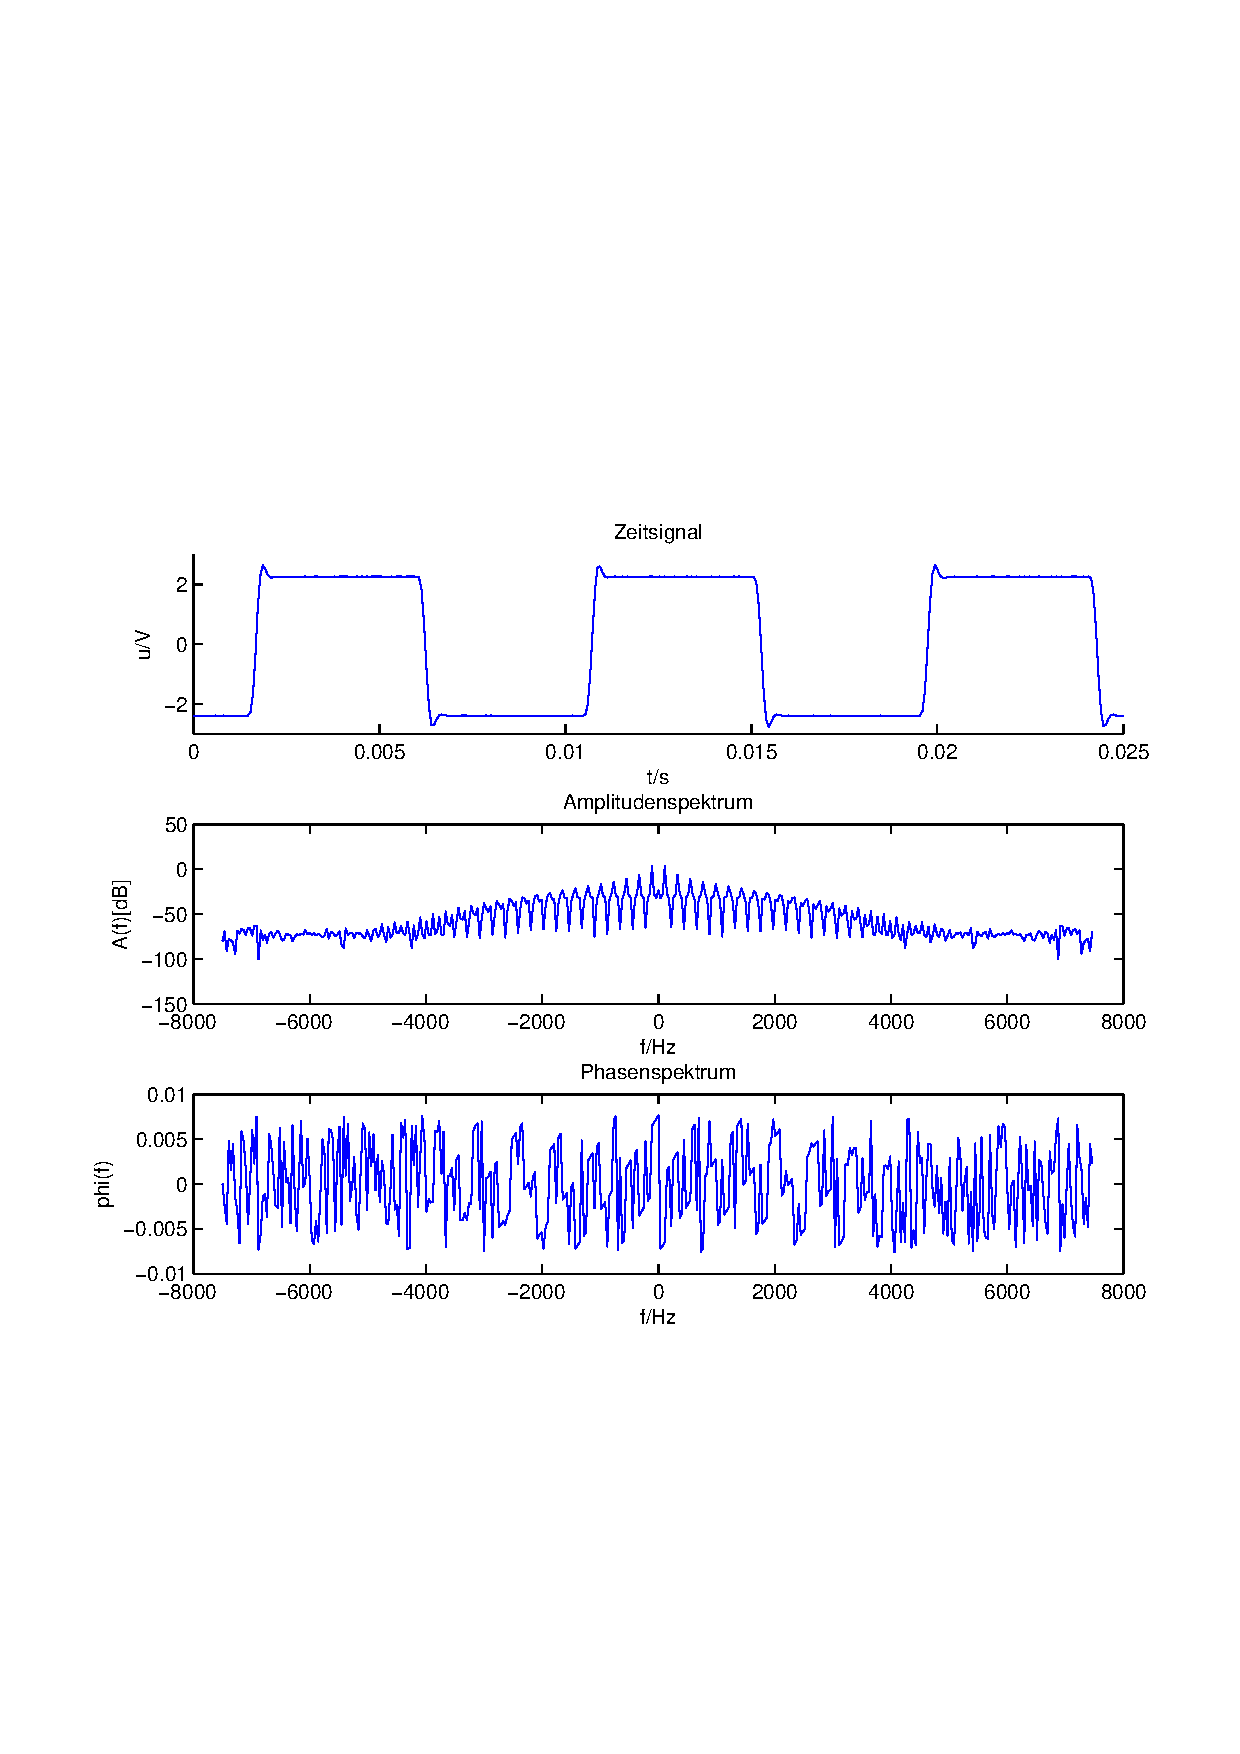
\includegraphics[scale=0.7, trim = 1.5cm 6.5cm 1cm 7.5cm,
                clip]{./Bilder/rechteck_100Hz_15kHz_keine_frequenzbegrenzung.pdf}
                    \caption{gesamtes Spektrum des aufgenommenen Rechtecks}
            \end{figure}
        
            Das Spektrum des nicht nachabgetasteten Signals verläuft bis ca. $7,5kHz$. Allerdings sind die
            Frequenzanteile in diesen Bereichen so minimal, dass sie in Messfehlern untergehen und keine Aussagekraft haben. Dennoch belegen sie Speicher.\\
            Diese Spektrallinien können vernachlässigt werden. Daher wird das Signal nachabgetastet.
            
            \begin{figure}[H]
            \centering
                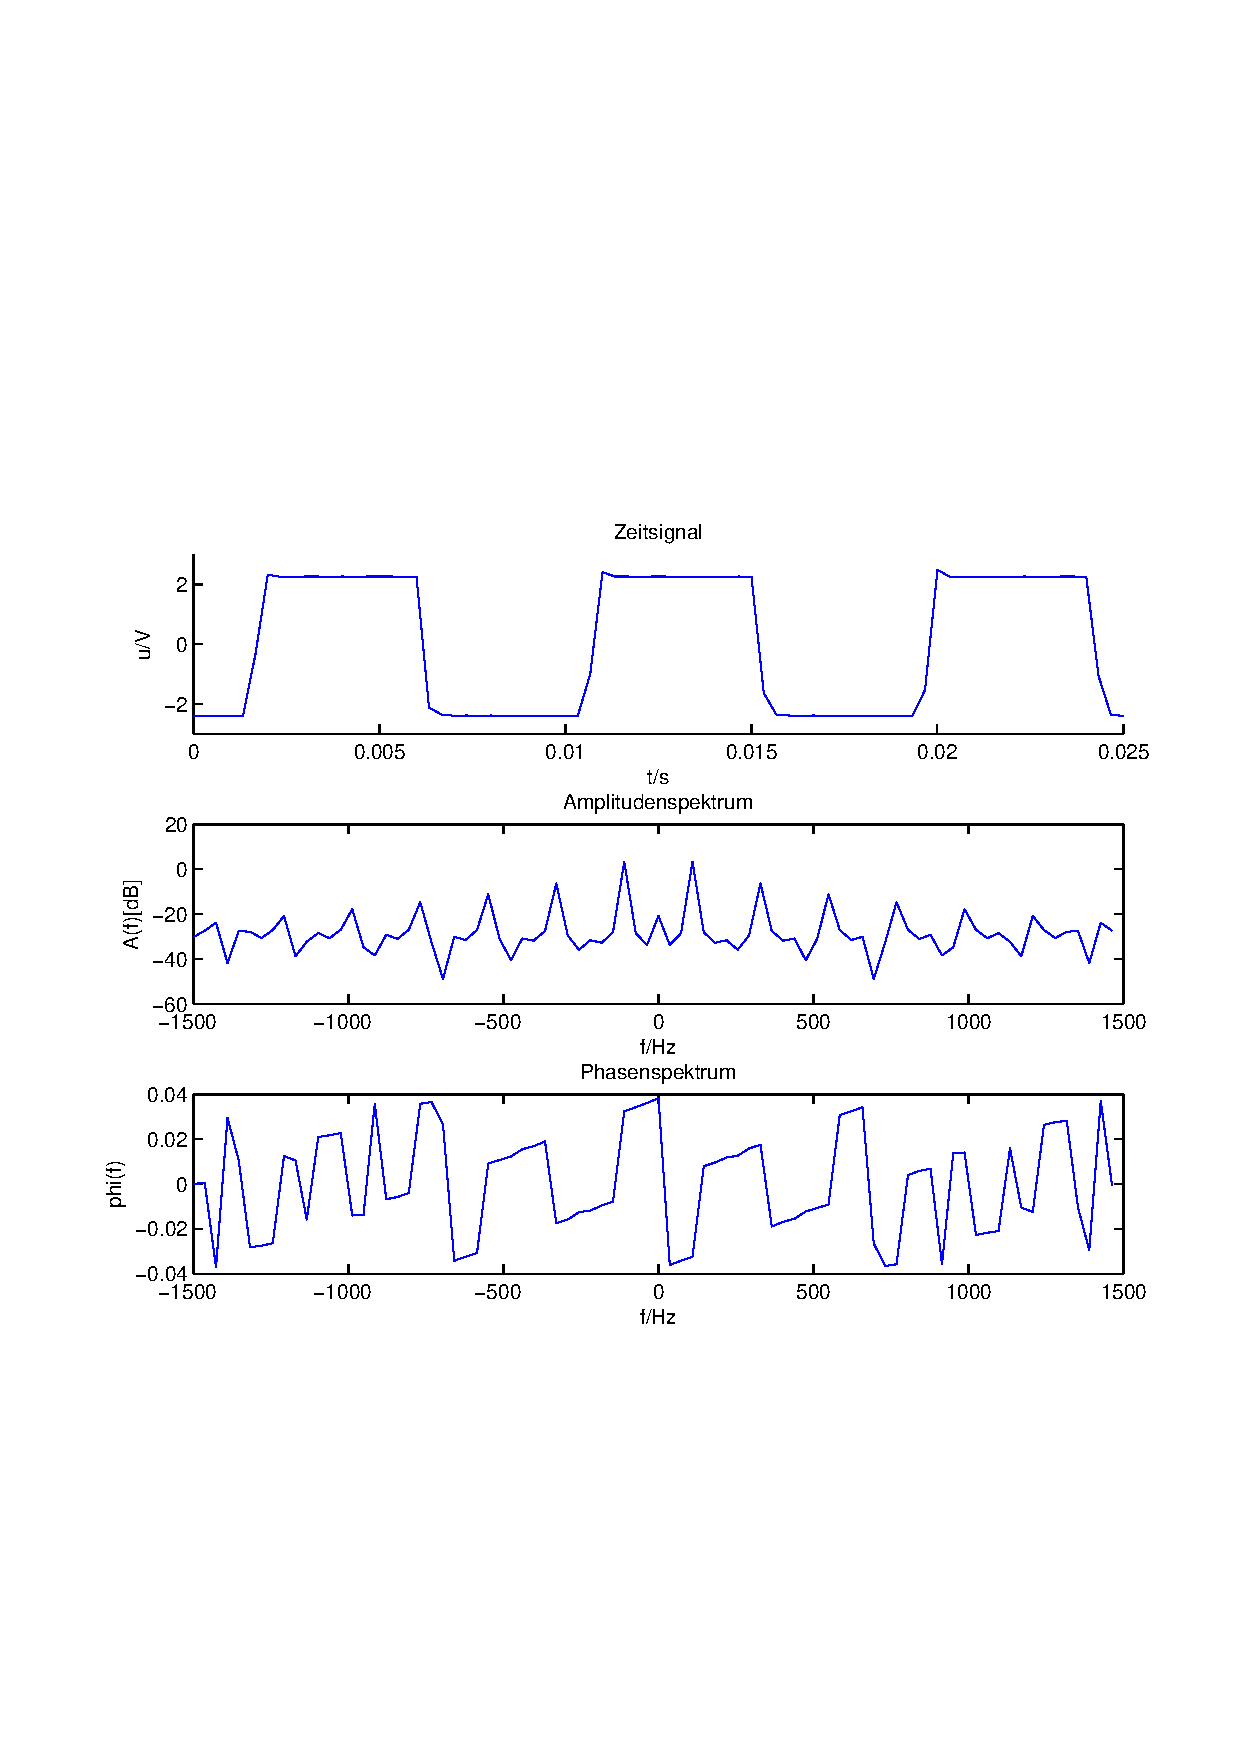
\includegraphics[scale=0.7, trim = 1.5cm 6.5cm 1cm 7.5cm,
                clip]{./Bilder/rechteck_100Hz_15kHz_3kHz_nachabgetastet_keine_frequenzbegrenzung.pdf}
                    \caption{gesamtes Spektrum des nachabgetasteten Signals}
            \end{figure}
        
            Das Spektrum des Nachabgetasteten Signals hat zwischen den einzelnen Spektrallinien den gleichen Abstand wie das Spektrum des 
            unbearbeiteten Signals. Allerdings fehlen die höheren Frequenzen, da diese nun nicht mehr mit einer Abtastfrequenz erfasst werden 
            können, die geringer ist als sie selbst. Daher ist das Spektrum des nachabgetasteten Signals nun schmaler als die des ursprünglichen 
            Messsignals.\\
        
            Da die wichtigen Spektrallinien im Bereich bis $1kHz$ liegen wird nun dieser Bereich betrachtet. In der
            Nachansicht des Spektrums fällt auf, das der Oberwellenanteil im Spektrum leicht gestiegen ist.\\
            Diese Frequenzanteile entstehen durch die Nachabtastung. Bei der Nachabtastung des $7,5kHz$ Signals, wird
            das Signal mit einer Frequenz von $3kHz$ abgetastet. Dadurch kommt es zu Allaising. Dies ist aber nicht von
            Bedeutung, da diese Frequenzanteile sehr gering sind. Die Verfälschung des Spektrums ist sehr klein.
			
		\end{quote} % Ende Subsubsection Aufgabe 5.1
    \end{quote}  % Ende Subsection Auswertung Termin 5
    
    \subsection{Auswertung Termin 6}
    \begin{quote}
        
        \subsubsection{Zusatzaufgabe: Messung der Dauer}
		\begin{quote}
			Mit Matlab wird eine Messung gestartet. Dadurch wird im Verlauf der Messung mehrfach die 
            Funktion filterFIRDecim aufgerufen. Dabei wird bei jedem Durchlauf
            ein Impuls erzeugt. Da die Funktion in kurzer Zeit mehrfach hintereinander aufgerufen wird, 
            kann mit dem Oszilloskop ein annähernd periodisches Signal
            beobachtet werden. Mit der Run/Stop-Taster kann die Messung festgehalten werden. 
            Die Dauer für einen Durchlauf kann nun am Oszilloskop abgelesen
            werden.\\
        
            \begin{figure}[H]
            \centering
                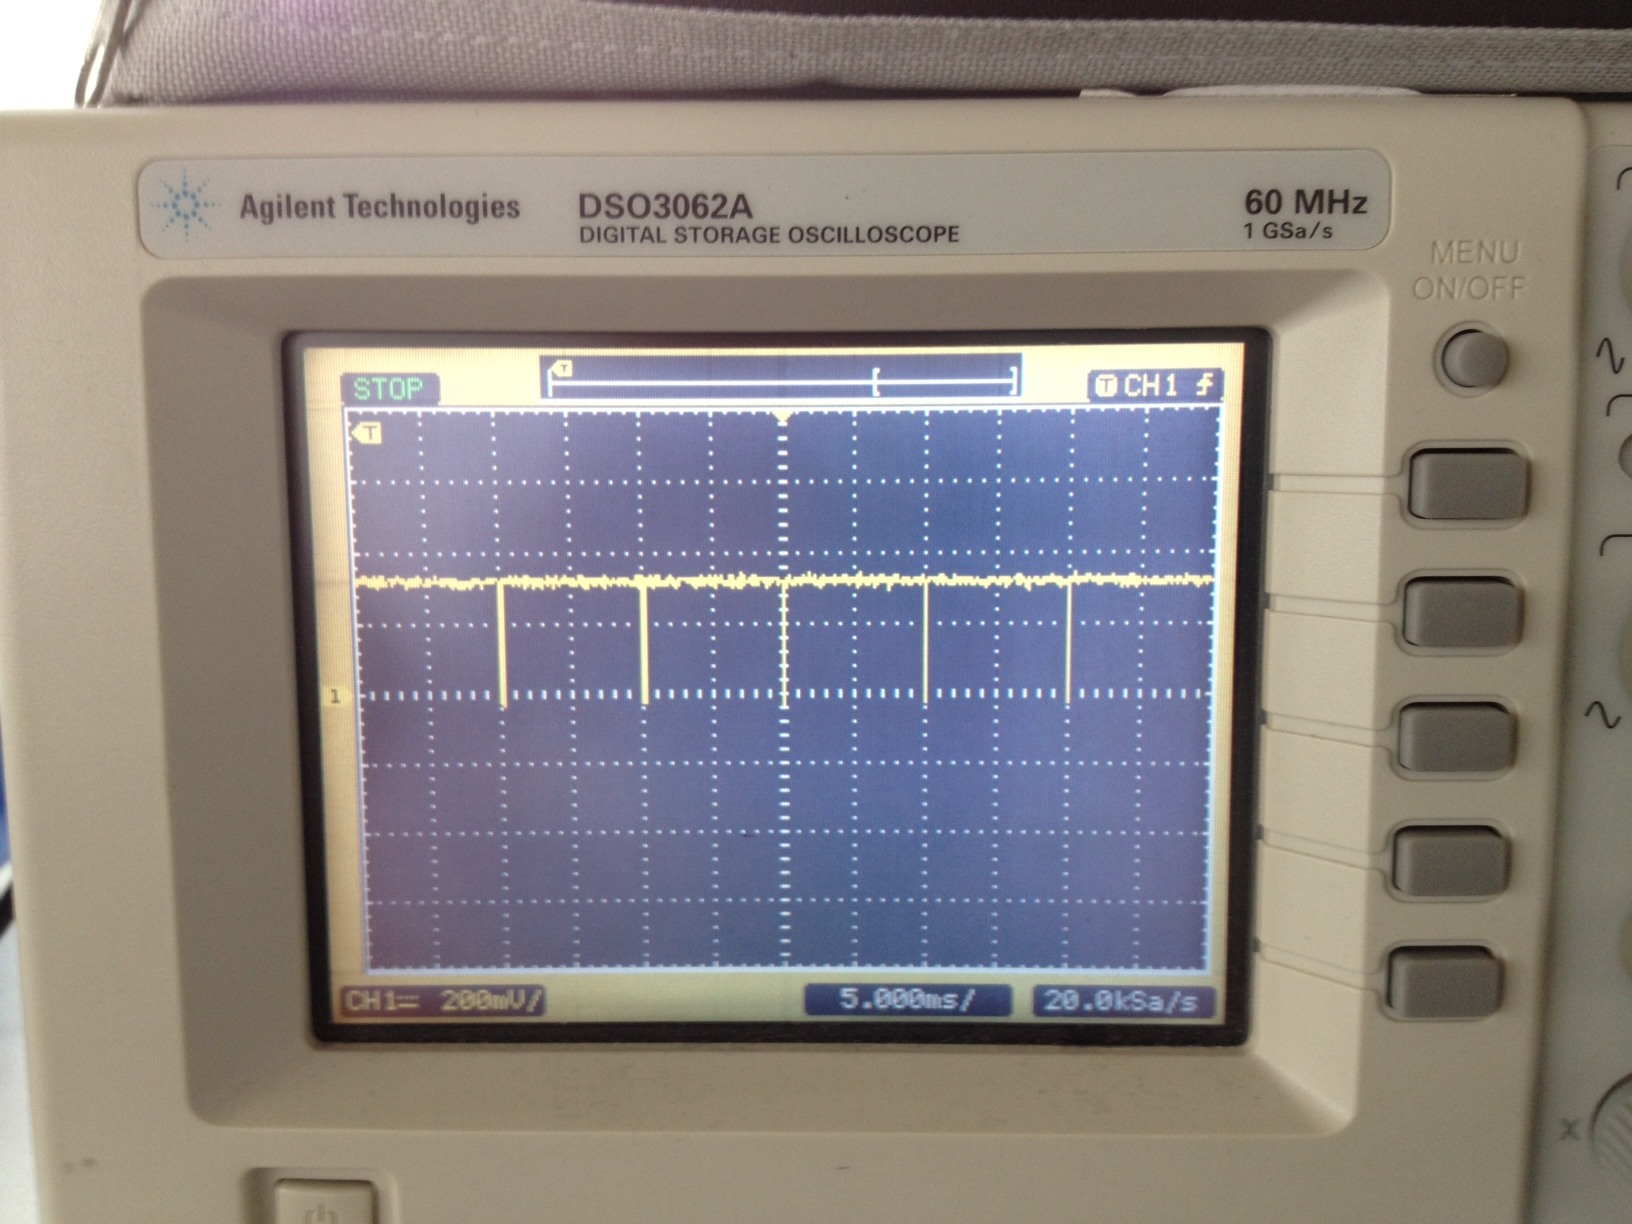
\includegraphics[scale=0.2, trim = 0cm 0cm 0cm 0cm, clip]{./Bilder/Foto.jpg}
                    \caption{Messung mit dem Oszilloskop}
            \end{figure}
        
            Ein Durchlauf von filterFIRDecim dauert $10ms$.
            
		\end{quote} % Ende Subsubsection Zusatzaufgabe
        
    \end{quote}  % Ende Subsection Auswertung Termin 6
\end{quote} %Ende section

%--------------------------------------------------------------------
%--------------------------------------------------------------------    


%--------------------------------------------------------------------
%--------------------------------------------------------------------
\section{Quellcodes}
\begin{quote}

	\subsection{Codes aus Termin 5}
	\begin{quote}
	    \subsubsection{FIRfilterung.m}
	    \begin{quote}
	        \lstinputlisting[
	            caption={FIRfilterung},
	            label=lst:Matlab]
	            {./Matlab/FIRfilterung.m}
	    \end{quote}
	    
	    \subsubsection{getFIRTiefpass.m}
	    \begin{quote}
	        \lstinputlisting[
	            caption={getFIRTiefpass},
	            label=lst:Matlab]
	            {./Matlab/getFIRTiefpass.m}
	    \end{quote}

        \subsubsection{Testfunktion.m}
        \begin{quote}
            \lstinputlisting[
                caption={Testfunktion},
                label=lst:Matlab]
                {./Matlab/Testfunktion.m}
        \end{quote}
	    
	    \subsubsection{DecimFilt.m}
	    \begin{quote}
	        \lstinputlisting[
	            caption={DecimFilt},
	            label=lst:Matlab]
	            {./Matlab/DecimFilt.m}
	    \end{quote}
	    
	\end{quote}
\end{quote}

%--------------------------------------------------------------------
%--------------------------------------------------------------------


%\begin{thebibliography}{999}
%\bibitem {Schaltungwandlerbox} Prof. Dr.-Ing. Gühmann, Clemens; Dipl.-Ing. Funk, Jürgen: MDVLaborGeraete_web, S.4

%Name, Vorname.; evtl. Name2, Vorname2.: Titel des Dokumentes
%oder Buches, Zeitschrift/Verlag/URL (Auflage, Erscheinungsort, -jahr), ggf. Seitenzahlen
%\bibitem {PasevalscheTheorem} \url{https://de.wikipedia.org/wiki/Parsevalsches_Theorem}, Zugriff
%23.05.2012
%\end{thebibliography}


\end{document}


